\documentclass{article}\usepackage[]{graphicx}\usepackage[]{color}
%% maxwidth is the original width if it is less than linewidth
%% otherwise use linewidth (to make sure the graphics do not exceed the margin)
\makeatletter
\def\maxwidth{ %
  \ifdim\Gin@nat@width>\linewidth
    \linewidth
  \else
    \Gin@nat@width
  \fi
}
\makeatother

\definecolor{fgcolor}{rgb}{0.345, 0.345, 0.345}
\newcommand{\hlnum}[1]{\textcolor[rgb]{0.686,0.059,0.569}{#1}}%
\newcommand{\hlstr}[1]{\textcolor[rgb]{0.192,0.494,0.8}{#1}}%
\newcommand{\hlcom}[1]{\textcolor[rgb]{0.678,0.584,0.686}{\textit{#1}}}%
\newcommand{\hlopt}[1]{\textcolor[rgb]{0,0,0}{#1}}%
\newcommand{\hlstd}[1]{\textcolor[rgb]{0.345,0.345,0.345}{#1}}%
\newcommand{\hlkwa}[1]{\textcolor[rgb]{0.161,0.373,0.58}{\textbf{#1}}}%
\newcommand{\hlkwb}[1]{\textcolor[rgb]{0.69,0.353,0.396}{#1}}%
\newcommand{\hlkwc}[1]{\textcolor[rgb]{0.333,0.667,0.333}{#1}}%
\newcommand{\hlkwd}[1]{\textcolor[rgb]{0.737,0.353,0.396}{\textbf{#1}}}%
\let\hlipl\hlkwb

\usepackage{framed}
\makeatletter
\newenvironment{kframe}{%
 \def\at@end@of@kframe{}%
 \ifinner\ifhmode%
  \def\at@end@of@kframe{\end{minipage}}%
  \begin{minipage}{\columnwidth}%
 \fi\fi%
 \def\FrameCommand##1{\hskip\@totalleftmargin \hskip-\fboxsep
 \colorbox{shadecolor}{##1}\hskip-\fboxsep
     % There is no \\@totalrightmargin, so:
     \hskip-\linewidth \hskip-\@totalleftmargin \hskip\columnwidth}%
 \MakeFramed {\advance\hsize-\width
   \@totalleftmargin\z@ \linewidth\hsize
   \@setminipage}}%
 {\par\unskip\endMakeFramed%
 \at@end@of@kframe}
\makeatother

\definecolor{shadecolor}{rgb}{.97, .97, .97}
\definecolor{messagecolor}{rgb}{0, 0, 0}
\definecolor{warningcolor}{rgb}{1, 0, 1}
\definecolor{errorcolor}{rgb}{1, 0, 0}
\newenvironment{knitrout}{}{} % an empty environment to be redefined in TeX

\usepackage{alltt}
\usepackage{breakurl}
\usepackage{graphicx, verbatim}
\usepackage{amsmath}
\usepackage{amscd}
\usepackage{lipsum}
\usepackage{enumitem}
\usepackage{todonotes}
\usepackage[tableposition=top]{caption}
\usepackage{ifthen}
\usepackage[utf8]{inputenc}
\usepackage{graphicx}
\usepackage{caption}
\usepackage{listings}
\usepackage{inconsolata}
\usepackage{url}
\setlength{\textwidth}{6.5in} 
\setlength{\textheight}{9in}
\setlength{\oddsidemargin}{0in} 
\setlength{\evensidemargin}{0in}
\setlength{\topmargin}{-1.5cm}
\setlength{\parindent}{0cm}
\usepackage{setspace}
\usepackage{float}
\usepackage{setspace}
\usepackage{float}
\usepackage{hyperref}
\hypersetup{
  colorlinks   = true, %Colours links instead of ugly boxes
  urlcolor     = blue, %Colour for external hyperlinks
  linkcolor    = blue, %Colour of internal links
  citecolor   = red %Colour of citations
}
\IfFileExists{upquote.sty}{\usepackage{upquote}}{}
\begin{document}
\title{CM3111 Big Data Coursework}
\author{Petar Bonchev}
\maketitle
\section{Data Exploration}
\begin{itemize}
\newline 1.1. Data choice
\newline 

\item 
\newline  The dataset I decided to use is Phishing websites provided by UCI machine learning repositoryhttps://archive.ics.uci.edu/ml/datasets/Phishing+Websites}.
\newline 
\item 
\newline  I chose this data set because of its practical potential to predict dangerouse websites for the user and also because the size of the dataset is more appropriate for the current coursework and of manageable size. In addition, hacking/ethical hacking have always been an interesting subject for me.

\newline 
\newline 1.2. Problem statement and Data Exploration
\newline 
\item
\newline In this dataset are presented one of the most famous and widely used features that have proved to be sound and effective in predicting phishing websites.  Each attribute corresponds to a particular technique that was used to determine whether the tested website falls into one of the three website caterogies - legimate, suspicious and phishing.
\newline 

\item 
\newline In this coursework the aim is to build a predictive model so it can predict which websites are phishing websites and contain malware harmful to the user.

\item
\newline As we can see below the names of the features(columns), each column stands for a different way a website can be detected whether it contains some kind of malware. Although, this data set contains data for 31 distinctive malware detecting methods, there is no agreement in literature on the definitive features that characterize phishing websites and it is difficult to shape a dataset that covers all possible features. In addition, in this data set some new features have been proposed, new rules have been experimentally assigned to some well-known features and some other features have been updated.
\newline

\end{itemize}
\newline
\newline
\newline
\newline
\newline
\begin{knitrout}
\definecolor{shadecolor}{rgb}{0.969, 0.969, 0.969}\color{fgcolor}\begin{kframe}
\begin{alltt}
\hlkwd{options}\hlstd{(}\hlkwc{scipen} \hlstd{=} \hlnum{999}\hlstd{)} \hlcom{# disable scientific notation -numbers}
\hlstd{cwFile} \hlkwb{<-} \hlkwd{read.csv}\hlstd{(}\hlstr{'C:\textbackslash{}\textbackslash{}Users\textbackslash{}\textbackslash{}Peter Boncheff\textbackslash{}\textbackslash{}Desktop\textbackslash{}\textbackslash{}Courseworks\textbackslash{}\textbackslash{}Big Data\textbackslash{}\textbackslash{}phishing.csv'}\hlstd{)}
\hlcom{# Read and save dataset}
\hlstd{df} \hlkwb{<-} \hlstd{cwFile} \hlcom{# use an alternative data frame}
\hlkwd{cat}\hlstd{(}\hlstr{"This phishing Websites database has"}\hlstd{,} \hlkwd{nrow}\hlstd{(df),} \hlstr{"rows and"}\hlstd{,} \hlkwd{ncol}\hlstd{(df),} \hlstr{"columns"}\hlstd{)}
\end{alltt}
\begin{verbatim}
## This phishing Websites database has 999 rows and 31 columns
\end{verbatim}
\begin{alltt}
\hlkwd{names}\hlstd{(df)} \hlcom{# illustrating all names of columns}
\end{alltt}
\begin{verbatim}
##  [1] "having_IP_Address"           "URL_Length"                 
##  [3] "Shortining_Service"          "having_At_Symbol"           
##  [5] "double_slash_redirecting"    "Prefix_Suffix"              
##  [7] "having_Sub_Domain"           "SSLfinal_State"             
##  [9] "Domain_registeration_length" "Favicon"                    
## [11] "port"                        "HTTPS_token"                
## [13] "Request_URL"                 "URL_of_Anchor"              
## [15] "Links_in_tags"               "SFH"                        
## [17] "Submitting_to_email"         "Abnormal_URL"               
## [19] "Redirect"                    "on_mouseover"               
## [21] "RightClick"                  "popUpWidnow"                
## [23] "Iframe"                      "age_of_domain"              
## [25] "DNSRecord"                   "web_traffic"                
## [27] "Page_Rank"                   "Google_Index"               
## [29] "Links_pointing_to_page"      "Statistical_report"         
## [31] "Result"
\end{verbatim}
\end{kframe}
\end{knitrout}
\begin{itemize}
\item 
\newline The data set is filled with integers all of which are either 1,0 or -1. These integers represent whether the method that was used to predict which websites are malicious(phishing). Therefore,
1 stands for legitimate website, 0 stands for suspicious website and -1 stands for phishing website.
\end{itemize}

\begin{knitrout}
\definecolor{shadecolor}{rgb}{0.969, 0.969, 0.969}\color{fgcolor}\begin{kframe}
\begin{alltt}
\hlkwd{str}\hlstd{(df)} \hlcom{# Quick description of the dataset;}
\end{alltt}
\begin{verbatim}
## 'data.frame':	999 obs. of  31 variables:
##  $ having_IP_Address          : int  -1 1 1 1 1 -1 1 1 1 1 ...
##  $ URL_Length                 : int  1 1 0 0 0 0 0 0 0 1 ...
##  $ Shortining_Service         : int  1 1 1 1 -1 -1 -1 1 -1 -1 ...
##  $ having_At_Symbol           : int  1 1 1 1 1 1 1 1 1 1 ...
##  $ double_slash_redirecting   : int  -1 1 1 1 1 -1 1 1 1 1 ...
##  $ Prefix_Suffix              : int  -1 -1 -1 -1 -1 -1 -1 -1 -1 -1 ...
##  $ having_Sub_Domain          : int  -1 0 -1 -1 1 1 -1 -1 1 -1 ...
##  $ SSLfinal_State             : int  -1 1 -1 -1 1 1 -1 -1 1 1 ...
##  $ Domain_registeration_length: int  -1 -1 -1 1 -1 -1 1 1 -1 -1 ...
##  $ Favicon                    : int  1 1 1 1 1 1 1 1 1 1 ...
##  $ port                       : int  1 1 1 1 1 1 1 1 1 1 ...
##  $ HTTPS_token                : int  -1 -1 -1 -1 1 -1 1 -1 -1 1 ...
##  $ Request_URL                : int  1 1 1 -1 1 1 -1 -1 1 1 ...
##  $ URL_of_Anchor              : int  -1 0 0 0 0 0 -1 0 0 0 ...
##  $ Links_in_tags              : int  1 -1 -1 0 0 0 0 -1 1 1 ...
##  $ SFH                        : int  -1 -1 -1 -1 -1 -1 -1 -1 -1 -1 ...
##  $ Submitting_to_email        : int  -1 1 -1 1 1 -1 -1 1 1 1 ...
##  $ Abnormal_URL               : int  -1 1 -1 1 1 -1 -1 1 1 1 ...
##  $ Redirect                   : int  0 0 0 0 0 0 0 0 0 0 ...
##  $ on_mouseover               : int  1 1 1 1 -1 1 1 1 1 1 ...
##  $ RightClick                 : int  1 1 1 1 1 1 1 1 1 1 ...
##  $ popUpWidnow                : int  1 1 1 1 -1 1 1 1 1 1 ...
##  $ Iframe                     : int  1 1 1 1 1 1 1 1 1 1 ...
##  $ age_of_domain              : int  -1 -1 1 -1 -1 1 1 -1 1 1 ...
##  $ DNSRecord                  : int  -1 -1 -1 -1 -1 1 -1 -1 -1 -1 ...
##  $ web_traffic                : int  -1 0 1 1 0 1 -1 0 1 0 ...
##  $ Page_Rank                  : int  -1 -1 -1 -1 -1 -1 -1 -1 1 -1 ...
##  $ Google_Index               : int  1 1 1 1 1 1 1 1 1 1 ...
##  $ Links_pointing_to_page     : int  1 1 0 -1 1 -1 0 0 0 0 ...
##  $ Statistical_report         : int  -1 1 -1 1 1 -1 -1 1 1 1 ...
##  $ Result                     : int  -1 -1 -1 -1 1 1 -1 -1 1 -1 ...
\end{verbatim}
\end{kframe}
\end{knitrout}

As we can see the distribution from the bar plot about 30 percent of the tested websites that have sub domains(see column -1) contain harmful malware, slighty more than 30 percent (see column 0) are suspicious and could harm the user and just over 40 percent are legitemate(see column 1). In addition, all numbers are integers, none are factors. 
\newline
\newline An example is given below of how the different techniques work to determine whether a website is phishing or legitemate. Since the data set consists of 31 attributes I thought it will be redundant if I explain how every single one works.
\newline 
\newline
Attribute - having\_IP\_Address
\newline

If an IP address is used as an alternative of the domain name in the URL, such as url{  http://125.98.3.123/fake.html}, users can be sure that someone is trying to steal their personal information. Sometimes, the IP address is even transformed into hexadecimal code as shown in the following link url{ http://0x58.0xCC.0xCA.0x62/2/paypal.ca/index.html}.
\newline
Rule: If The Domain Part has an IP Address - Phishing, Otherwise - Legitimate
\newline

\begin{knitrout}
\definecolor{shadecolor}{rgb}{0.969, 0.969, 0.969}\color{fgcolor}\begin{kframe}
\begin{alltt}
\hlkwd{par}\hlstd{(}\hlkwc{mar}\hlstd{=}\hlkwd{c}\hlstd{(}\hlnum{7.1}\hlstd{,} \hlnum{7.1}\hlstd{,} \hlnum{7.1}\hlstd{,} \hlnum{2.1}\hlstd{),}\hlkwc{mgp}\hlstd{=}\hlkwd{c}\hlstd{(}\hlnum{3}\hlstd{,} \hlnum{2}\hlstd{,} \hlnum{0}\hlstd{),}\hlkwc{las}\hlstd{=}\hlnum{0}\hlstd{)} \hlcom{#sets graphic grid to 2 by 2 with margin spacing}
\hlstd{labelFreqs} \hlkwb{<-} \hlkwd{table}\hlstd{(df}\hlopt{$}\hlstd{having_Sub_Domain)} \hlcom{# frequency of Result}
\hlkwd{barplot}\hlstd{(labelFreqs,}\hlkwc{col} \hlstd{=} \hlkwd{grey.colors}\hlstd{(}\hlnum{3}\hlstd{),} \hlcom{# Shows the frequency of having sub domain; }
        \hlkwc{main}\hlstd{=}\hlstr{"Websites that have sub domain"}\hlstd{)}
\end{alltt}
\end{kframe}
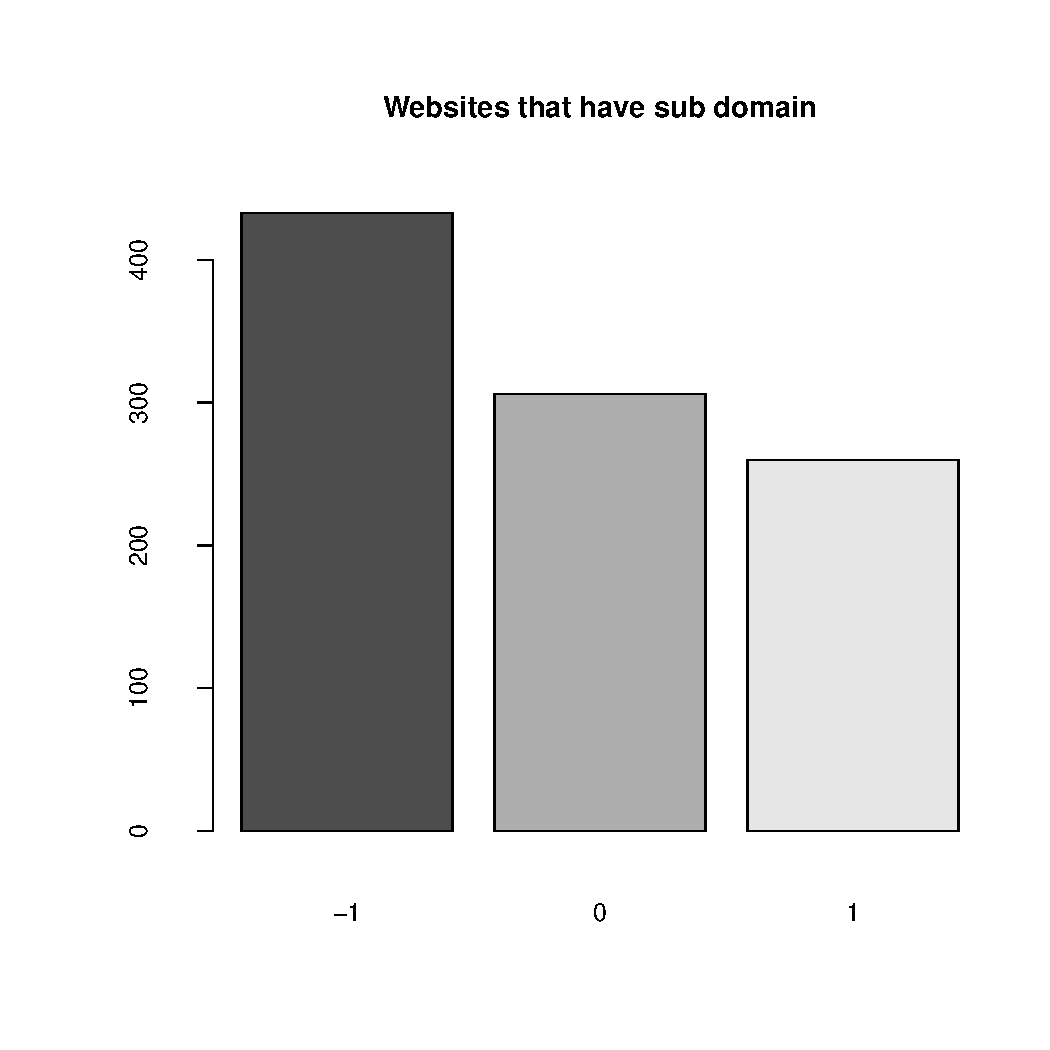
\includegraphics[width=\maxwidth]{figure/unnamed-chunk-3-1} 
\begin{kframe}\begin{alltt}
\hlcom{#An example of results using a technique that checks whether the websites have sub domain}
\end{alltt}
\end{kframe}
\end{knitrout}
\newline
\newline
\newline
\newline
\newline 1.3. Pre-processing
\begin{knitrout}
\definecolor{shadecolor}{rgb}{0.969, 0.969, 0.969}\color{fgcolor}\begin{kframe}
\begin{alltt}
 \hlkwd{colSums}\hlstd{(}\hlkwd{is.na}\hlstd{(df))} \hlcom{# check for missing values }
\end{alltt}
\begin{verbatim}
##           having_IP_Address                  URL_Length 
##                           0                           0 
##          Shortining_Service            having_At_Symbol 
##                           0                           0 
##    double_slash_redirecting               Prefix_Suffix 
##                           0                           0 
##           having_Sub_Domain              SSLfinal_State 
##                           0                           0 
## Domain_registeration_length                     Favicon 
##                           0                           0 
##                        port                 HTTPS_token 
##                           0                           0 
##                 Request_URL               URL_of_Anchor 
##                           0                           0 
##               Links_in_tags                         SFH 
##                           0                           0 
##         Submitting_to_email                Abnormal_URL 
##                           0                           0 
##                    Redirect                on_mouseover 
##                           0                           0 
##                  RightClick                 popUpWidnow 
##                           0                           0 
##                      Iframe               age_of_domain 
##                           0                           0 
##                   DNSRecord                 web_traffic 
##                           0                           0 
##                   Page_Rank                Google_Index 
##                           0                           0 
##      Links_pointing_to_page          Statistical_report 
##                           0                           0 
##                      Result 
##                           0
\end{verbatim}
\end{kframe}
\end{knitrout}
\begin{itemize}
\item
\newline From the output above we can conclude that there are no missing values in the dataset. Therefore, techniques to predict the missing values are not required
\item
\newline Standarise or normalise 
\newline

\begin{knitrout}
\definecolor{shadecolor}{rgb}{0.969, 0.969, 0.969}\color{fgcolor}\begin{kframe}
\begin{alltt}
\hlcom{#standardize and normalise}
\hlstd{dat} \hlkwb{<-} \hlkwd{data.frame}\hlstd{(}\hlkwc{x} \hlstd{=} \hlkwd{rnorm}\hlstd{(}\hlnum{10}\hlstd{,} \hlnum{30}\hlstd{,} \hlnum{.2}\hlstd{),} \hlkwc{y} \hlstd{=} \hlkwd{runif}\hlstd{(}\hlnum{10}\hlstd{,} \hlnum{3}\hlstd{,} \hlnum{5}\hlstd{))}
\hlstd{scaled.dat} \hlkwb{<-} \hlkwd{scale}\hlstd{(dat)}

\hlcom{# check that we get mean of 0 and sd of 1}
\hlkwd{colMeans}\hlstd{(scaled.dat)}  \hlcom{# a version of apply(scaled.dat, 2, mean)}
\end{alltt}
\begin{verbatim}
##                          x                          y 
##  0.00000000000000002498002 -0.00000000000000025374668
\end{verbatim}
\begin{alltt}
\hlkwd{apply}\hlstd{(scaled.dat,} \hlnum{2}\hlstd{, sd)}
\end{alltt}
\begin{verbatim}
## x y 
## 1 1
\end{verbatim}
\end{kframe}
\end{knitrout}

\newline From the results above we can conclude that the mean is 1 and so is the standard deviation, thus the data values are equal or really close to the mean which is easily observable since the data
only consists of -1,0, and 1.
\newline
\newline
\newline
\newline
\newline Generate or drop features
\newline
\newline Since the data is really well structured with no redundancy, there is no need to generate new features or to drop any of the current ones.

\end{itemize}

\section{Modelling/Classification}
\begin{itemize}
\item Vital part of modelling is to separate the given dataset into for example, one training and one testing subset. In this section, I divide the data into a training and a testing subsets, build a model with the training set and finally test,evaluate and discuss the results.
\end{itemize}

\newline 2.1. Divide data
\begin{knitrout}
\definecolor{shadecolor}{rgb}{0.969, 0.969, 0.969}\color{fgcolor}\begin{kframe}
\begin{alltt}
\hlkwd{library}\hlstd{(dplyr)}
\hlkwd{library}\hlstd{(caret)}
\hlkwd{library}\hlstd{(ISLR)}

\hlstd{idTrain} \hlkwb{<-} \hlkwd{createDataPartition}\hlstd{(df}\hlopt{$}\hlstd{Result,} \hlkwc{p}\hlstd{=}\hlnum{0.7}\hlstd{,}\hlkwc{list}\hlstd{=}\hlnum{FALSE}\hlstd{,} \hlkwc{times}\hlstd{=}\hlnum{1}\hlstd{)}
\hlcom{# dividing the data 70% training set and 30% test set}
\hlstd{train} \hlkwb{<-} \hlstd{df[idTrain,]} \hlcom{# training set with p = 0.7}
\hlstd{sid} \hlkwb{<-} \hlkwd{as.numeric}\hlstd{(}\hlkwd{rownames}\hlstd{(train))}
\hlstd{test} \hlkwb{<-} \hlstd{df[}\hlopt{-}\hlstd{sid,]} \hlcom{# test set with p = 0.3}
\end{alltt}
\end{kframe}
\end{knitrout}

\newline 2.2. Test and Evaluate

\begin{knitrout}
\definecolor{shadecolor}{rgb}{0.969, 0.969, 0.969}\color{fgcolor}\begin{kframe}
\begin{alltt}
\hlkwd{set.seed}\hlstd{(}\hlnum{99}\hlstd{)} \hlcom{#set seed for reproducibility}
\hlkwd{library}\hlstd{(randomForest)} \hlcom{# using randomforest libarary}
\hlkwd{prop.table}\hlstd{(}\hlkwd{table}\hlstd{(train}\hlopt{$}\hlstd{Result))}
\end{alltt}
\begin{verbatim}
## 
##        -1         1 
## 0.4414286 0.5585714
\end{verbatim}
\begin{alltt}
\hlstd{ctrl} \hlkwb{=} \hlkwd{trainControl}\hlstd{(}\hlkwc{method} \hlstd{=} \hlstr{"cv"}\hlstd{,} \hlkwc{number} \hlstd{=} \hlnum{5}\hlstd{)} \hlcom{#using cross validation to go through the dataset which is separated into 5(number = 5);}
\hlstd{train}\hlopt{$}\hlstd{Result} \hlkwb{=} \hlkwd{as.factor}\hlstd{(train}\hlopt{$}\hlstd{Result)}\hlcom{# convert the numbers to factors }
\hlstd{df}\hlopt{$}\hlstd{Result} \hlkwb{=} \hlkwd{ifelse}\hlstd{(df}\hlopt{$}\hlstd{Result} \hlopt{== -}\hlnum{1}\hlstd{,}\hlnum{0}\hlstd{,}\hlnum{1}\hlstd{)} \hlcom{# make the numbers be only 0 and 1(instead of -1 and 1)}
\hlstd{df}\hlopt{$}\hlstd{Result} \hlkwb{=} \hlkwd{as.factor}\hlstd{(df}\hlopt{$}\hlstd{Result)} \hlcom{# convert the numbers to factors in the main dataframe}
\hlstd{fitModel} \hlkwb{<-} \hlkwd{train}\hlstd{(Result}\hlopt{~}\hlstd{.,} \hlcom{#create a model}
                  \hlkwc{data}\hlstd{=train,} \hlcom{# data is set to be equal to train}
                  \hlkwc{method}\hlstd{=}\hlstr{"rf"}\hlstd{,} \hlcom{#using randomforest algorithm}
                  \hlkwc{trControl}\hlstd{=ctrl,}
                  \hlkwc{ntree} \hlstd{=} \hlnum{5}\hlstd{)} \hlcom{# number of trees}

\hlstd{pred} \hlkwb{<-} \hlkwd{predict}\hlstd{(fitModel, test[,}\hlopt{-}\hlkwd{ncol}\hlstd{(test)])} \hlcom{#predict that dataset}
\hlstd{test} \hlkwb{<-} \hlkwd{cbind}\hlstd{(test,pred)} \hlcom{#bind predictions}
\hlstd{results} \hlkwb{<-} \hlkwd{confusionMatrix}\hlstd{(}\hlkwd{table}\hlstd{(test}\hlopt{$}\hlstd{pred, test}\hlopt{$}\hlstd{Result))}
\hlstd{accuracy} \hlkwb{<-} \hlkwd{sum}\hlstd{(}\hlkwd{diag}\hlstd{(results}\hlopt{$}\hlstd{table))}\hlopt{/}\hlkwd{nrow}\hlstd{(test)}
\hlkwd{cat}\hlstd{(}\hlstr{'Accuracy is '}\hlstd{, accuracy)} \hlcom{# show results}
\end{alltt}
\begin{verbatim}
## Accuracy is  0.9063545
\end{verbatim}
\end{kframe}
\end{knitrout}
As a class variable we use 'Result' which contains only 1 and -1, where 1 stands for legitimate website and -1 for phishing website.
\newline
\newline
\newline
\newline
\newline 2.3. Report and discuss results
\begin{knitrout}
\definecolor{shadecolor}{rgb}{0.969, 0.969, 0.969}\color{fgcolor}\begin{kframe}
\begin{alltt}
\hlcom{#Illustration and explaination .......}
\hlkwd{print}\hlstd{(fitModel)}
\end{alltt}
\begin{verbatim}
## Random Forest 
## 
## 700 samples
##  30 predictor
##   2 classes: '-1', '1' 
## 
## No pre-processing
## Resampling: Cross-Validated (5 fold) 
## Summary of sample sizes: 560, 560, 560, 560, 560 
## Resampling results across tuning parameters:
## 
##   mtry  Accuracy   Kappa    
##    2    0.8671429  0.7271435
##   16    0.9085714  0.8149341
##   30    0.9185714  0.8351717
## 
## Accuracy was used to select the optimal model using the largest value.
## The final value used for the model was mtry = 30.
\end{verbatim}
\begin{alltt}
\hlstd{aLabel} \hlkwb{<-} \hlkwd{table}\hlstd{(df}\hlopt{$}\hlstd{Result)} \hlcom{# frequency of Result}
\hlkwd{barplot}\hlstd{(aLabel,}\hlkwc{col} \hlstd{=} \hlkwd{grey.colors}\hlstd{(}\hlnum{3}\hlstd{),}
        \hlkwc{main}\hlstd{=}\hlstr{"Results after modelling and predicting"}\hlstd{)}
\end{alltt}
\end{kframe}
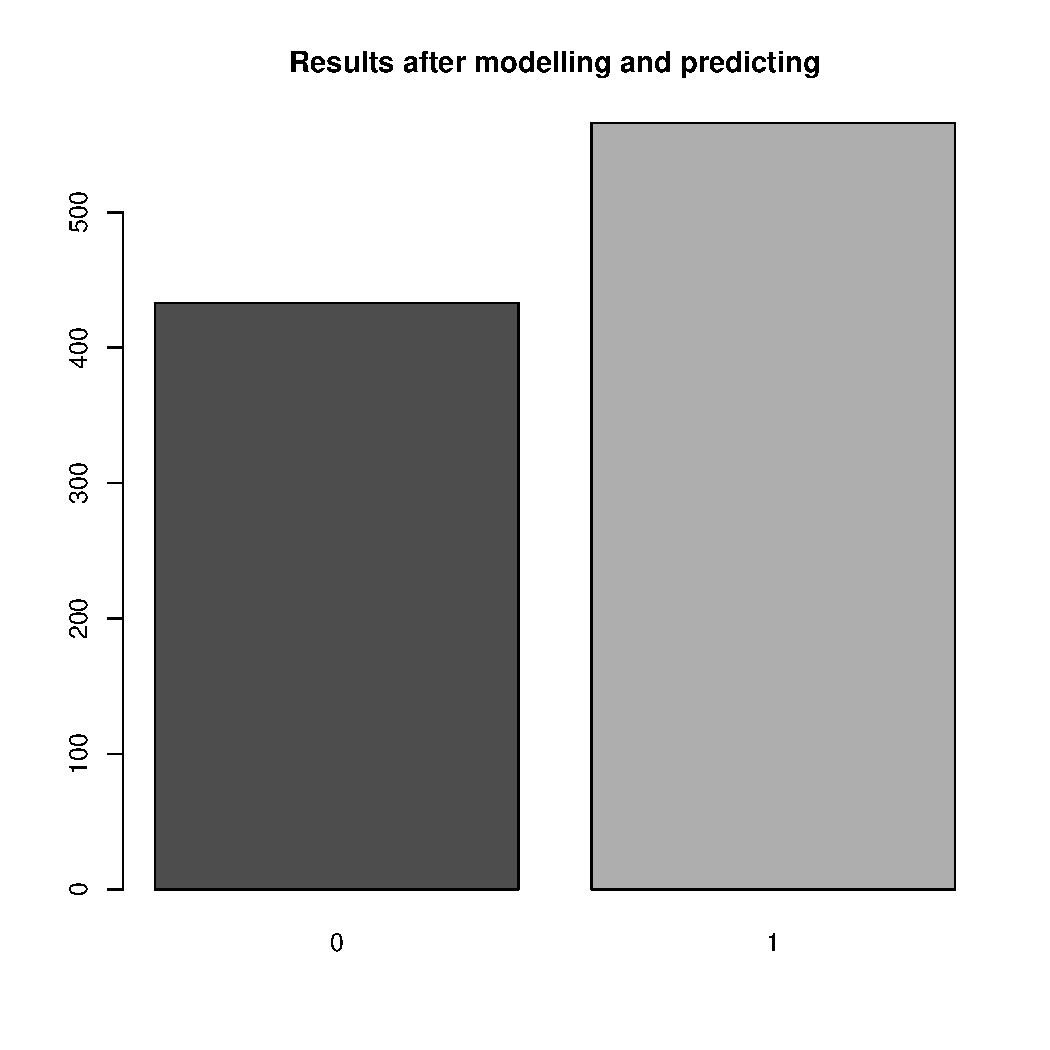
\includegraphics[width=\maxwidth]{figure/unnamed-chunk-8-1} 

\end{knitrout}
From the barplot above we can observe that the dataset is balanced and we are able to predict whether a website contains malware with approximately ninety percent accuracy.

\section{Improving performance}

\newline 3.1. Tune parameters & change partitioning of the dataset

\begin{knitrout}
\definecolor{shadecolor}{rgb}{0.969, 0.969, 0.969}\color{fgcolor}\begin{kframe}
\begin{alltt}
\hlstd{idTrainTwo} \hlkwb{<-} \hlkwd{createDataPartition}\hlstd{(df}\hlopt{$}\hlstd{Result,} \hlkwc{p}\hlstd{=}\hlnum{0.8}\hlstd{,}\hlkwc{list}\hlstd{=}\hlnum{FALSE}\hlstd{,} \hlkwc{times}\hlstd{=}\hlnum{1}\hlstd{)}
\hlcom{# this time we are dividing the data into a 80% training set and a 20% test set}

\hlstd{trainTwo} \hlkwb{<-} \hlstd{df[idTrainTwo,]} \hlcom{# training set with p = 0.8}
\hlstd{sid} \hlkwb{<-} \hlkwd{as.numeric}\hlstd{(}\hlkwd{rownames}\hlstd{(trainTwo))}
\hlstd{testTwo} \hlkwb{<-} \hlstd{df[}\hlopt{-}\hlstd{sid,]} \hlcom{# test set with p = 0.2}
\hlkwd{set.seed}\hlstd{(}\hlnum{201}\hlstd{)}
\hlkwd{prop.table}\hlstd{(}\hlkwd{table}\hlstd{(trainTwo}\hlopt{$}\hlstd{Result))}
\end{alltt}
\begin{verbatim}
## 
##       0       1 
## 0.43375 0.56625
\end{verbatim}
\end{kframe}
\end{knitrout}

\newline 3.2. Different models

\begin{knitrout}
\definecolor{shadecolor}{rgb}{0.969, 0.969, 0.969}\color{fgcolor}\begin{kframe}
\begin{alltt}
\hlstd{ctrlTwo} \hlkwb{=} \hlkwd{trainControl}\hlstd{(}\hlkwc{method} \hlstd{=} \hlstr{"cv"}\hlstd{,} \hlkwc{number} \hlstd{=} \hlnum{10}\hlstd{)}
\hlcom{# increasing the number variable by 5 (the previous model in section two is just 5)}
\hlstd{trainTwo}\hlopt{$}\hlstd{Result} \hlkwb{=} \hlkwd{as.factor}\hlstd{(trainTwo}\hlopt{$}\hlstd{Result)}
\hlstd{fitModelTwo} \hlkwb{<-} \hlkwd{train}\hlstd{(Result}\hlopt{~}\hlstd{.,}
                  \hlkwc{data}\hlstd{=trainTwo,}
                  \hlkwc{method}\hlstd{=}\hlstr{"rf"}\hlstd{,} \hlcom{# again with random forest}
                  \hlkwc{trControl}\hlstd{=ctrlTwo,}
                  \hlkwc{ntree}\hlstd{=}\hlnum{201}\hlstd{)}
\hlcom{# increasing the number of trees to be with 196 more than the one in the previous model}

\hlstd{predTwo} \hlkwb{<-} \hlkwd{predict}\hlstd{(fitModelTwo, testTwo[,}\hlopt{-}\hlkwd{ncol}\hlstd{(testTwo)])} \hlcom{#predict using the new model}
\hlstd{testTwo} \hlkwb{<-} \hlkwd{cbind}\hlstd{(testTwo,predTwo)}
\hlstd{resultsTwo} \hlkwb{<-} \hlkwd{confusionMatrix}\hlstd{(}\hlkwd{table}\hlstd{(testTwo}\hlopt{$}\hlstd{predTwo, testTwo}\hlopt{$}\hlstd{Result))}
\hlstd{accuracyTwo} \hlkwb{<-} \hlkwd{sum}\hlstd{(}\hlkwd{diag}\hlstd{(resultsTwo}\hlopt{$}\hlstd{table))}\hlopt{/}\hlkwd{nrow}\hlstd{(testTwo)}
\hlkwd{cat}\hlstd{(}\hlstr{'Accuracy is '}\hlstd{, accuracyTwo)}
\end{alltt}
\begin{verbatim}
## Accuracy is  0.9497487
\end{verbatim}
\begin{alltt}
\hlkwd{print}\hlstd{(fitModelTwo)}
\end{alltt}
\begin{verbatim}
## Random Forest 
## 
## 800 samples
##  30 predictor
##   2 classes: '0', '1' 
## 
## No pre-processing
## Resampling: Cross-Validated (10 fold) 
## Summary of sample sizes: 720, 720, 720, 721, 720, 720, ... 
## Resampling results across tuning parameters:
## 
##   mtry  Accuracy   Kappa    
##    2    0.9275733  0.8517811
##   16    0.9274953  0.8523839
##   30    0.9237920  0.8447274
## 
## Accuracy was used to select the optimal model using the largest value.
## The final value used for the model was mtry = 2.
\end{verbatim}
\end{kframe}
\end{knitrout}
We can observe that the accuracy has increased slightly by making the changes we made. Increasing the number of decision trees(from 5 to 201) helps to increase the precision of the algorithm.
\newline
\newline Conclusion 
\newline
\newline The above illustrates that the random forest manages to predict extremely well whether a website contains malware with approximately 90 percent accuracy. Increasing the number of decision trees and cross validation split number increases the accuracy slightly.
\end{document}

